\documentclass[a4paper,12pt]{article} % тип документа

% report, book



%  Русский язык

\usepackage[T2A]{fontenc}			% кодировка
\usepackage[utf8]{inputenc}			% кодировка исходного текста
\usepackage[english,russian]{babel}	% локализация и переносы
\usepackage{graphicx}
\graphicspath{{./}}
\DeclareGraphicsExtensions{.png,.jpg}


% Математика
\usepackage{amsmath,amsfonts,amssymb,amsthm,mathtools} 


\usepackage{wasysym}

%Заговолок
\author{Бредихин Александр}
\title{Домашняя работа №1}



\begin{document} % начало документа

\maketitle

\section*{Задача 1}

\begin{itemize}
\item \textbf{a)}  $n = \mathcal{O}(n\log{}n)$ - верно\\
$\square$ По определению:\\
$f(n) = \mathcal{O}(g(n)) \Leftrightarrow \exists C>0, \exists N\in\mathbb{N} : \forall n \geq N \rightarrow f(n) < C \cdot g(n)$\\
В нашем случае для функций $f(n) = n$ и $g(n) = n\log{}n$ выражение имеет вид:\
$n \leq Cn\log{}n \Longleftrightarrow 1 \leq C\log{}n$\\
Возьмём $C=1$ и N равное основанию логарифма. Тогда определение написанное выше верно, то есть логарифм больше либо равен константе. Следоватедьно $n = \mathcal{O}(n\log{}n)$ - верно по определению.
\begin{flushright}
	$\blacksquare$
\end{flushright}

\item \textbf{b)} $\exists\varepsilon > 0: n\log{}n = \Omega(n^{1+\varepsilon})$ - не верно.\\
$\square$ Запишем отрицание определения $\Omega(g(n)) = f(n)$\\
$\forall c>0, \forall N\in\mathbb{N}: \exists n \geq N \rightarrow f(n) < C \cdot g(n)$\\
Для наших функций $ \forall\varepsilon: n\log{}n < C \cdot n^{1+\varepsilon} \longleftrightarrow \log{}n < Cn^{\varepsilon}$\\
Докажем это, пользуясь правилом Лопиталя\\
\[ \lim\limits_{n\to\infty}\frac{n^{\varepsilon}}{\log{}n} = \left[ \frac{\infty}{\infty} \right] = 
\lim\limits_{n\to\infty}\frac{\varepsilon n^{\varepsilon - 1}n}{1} = 
\lim\limits_{n\to\infty}\varepsilon n^{\varepsilon} = \infty \]
Значит,
$\forall c,\varepsilon >0, \forall N\in\mathbb{N}: \exists n \geq N \rightarrow \log{}n < Cn^{\varepsilon}$ - верно.\\
Из отрицания определения следует, что ответ <<нет, не верно>>
\begin{flushright}
	$\blacksquare$
\end{flushright}

\end{itemize}

\section*{Задача 2}
\textbf{a)} Ответ: Да, возможно, например\\
$ f(n) = n\log{}^2n $, $ g(n) = \log{}n \rightarrow
h(x) = n\log{}n $ для такого примера оценки из условия на функции $ f(n) $ и $ g(n) $ верны  \\
Значит, $ h(n) = \Theta(n\log{}n) $ - верно.\\
P.s. Всем известно, что $ \log{}n =  \mathcal{O}(n)$, но почему   $f(n) = n\log{}^2n = \mathcal{O}(n^2)$?\\
Это легко получить подсчитав предел используя правило Лопиталя и сделав несколько преобразований:\\
 $ n\log{}^2n \leq n^2 \Leftrightarrow 
\log{}^2n \leq n \longmapsto 
 \lim\limits_{n\to\infty}\frac{n}{\log{}^2n} =
\left[ \frac{\infty}{\infty} \right] = 
\lim\limits_{n\to\infty}\frac{n}{2\log{}n} = 
\left[ \frac{\infty}{\infty} \right] = 
\lim\limits_{n\to\infty}\frac{n}{2} = \infty$   \\[1cm]
\textbf{b)} Из условия задачи $ f(n) \leq C_1n^2, g(n) \geq C_2, g(n) \leq C_3n $\\
Значит верхняя оценка для функции $ h(n) $ такая:\\
$ h(n) \leq \frac{f(n)}{g(n)} \leq \frac{C_1n^2}{C_2} \Longrightarrow 
h(n) = \mathcal{O}(n^2)$\\
А хотим получить: $ C'n^3 \leq h(n) \leq C''n^3 $. Из определения $ \mathcal{O}(n^2) $ получаем, что такой $ h(n) $ не существует.\\
Ответ: не возможно\\[1cm]
Верхнюю оценку на $ h(n) $ мы получили в пункте b): $ h(n) = \mathcal{O}(n^2)  $. Она достигается, например, когда $ f(n) = 2n^2, g(n) = 2 $ \\
Нижний оценки на $h(n)$ не существует, так как функция $ f(n) $ не ограничена снизу.

\section*{Задача 3}
$S(n) = \sum\limits_{i=1}^{n} \sqrt{i^{3}+2 i+5}=\sum\limits_{i=1}^{n} f(i)$\\
Аналогично семинарскому занятию, если мы построим график $f(n)$ от $ n $, то площадь под этим графиком оценивается $ S(n) $ (см. рисунок). 

\begin{center}
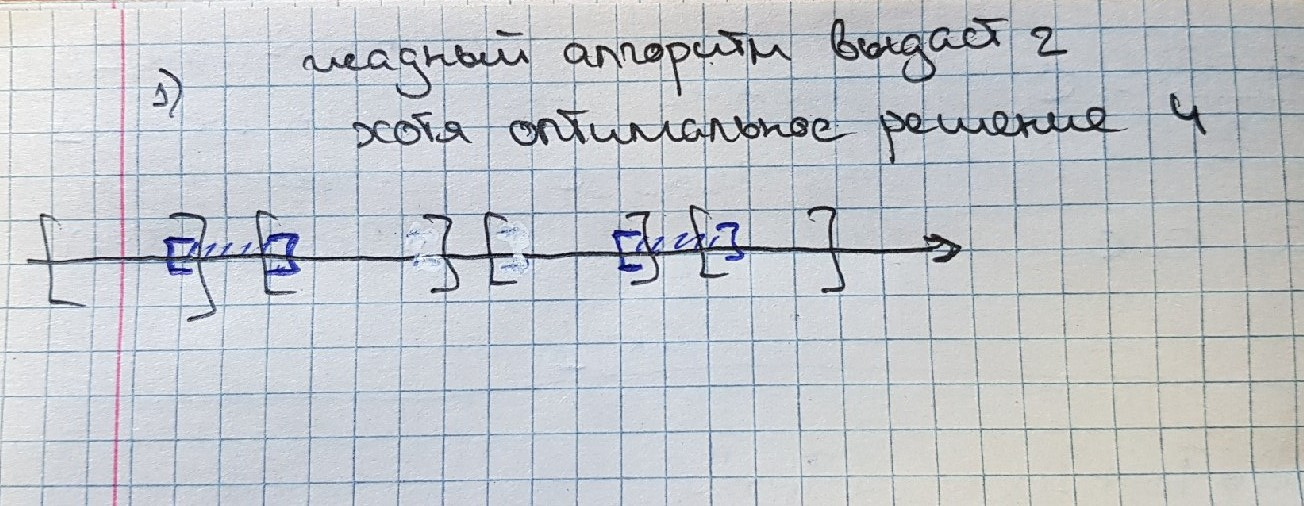
\includegraphics[width=0.7\textwidth]{pic_1}
\end{center}
Её можно оценить сверху большим прямоугольником размером $ n $ и $f(n)$. То есть\\
$ S(n) = \mathcal{O}(n \cdot f(n)) = \mathcal{O}(n^{\frac{5}{2}})$\\ так как $ S(n) \leq n \cdot \sqrt{n^{3}+2 \cdot n+5} \leq n \cdot n^{3 / 2}=n^{5 / 2} $\\
Снизу можно оценить прямоугольником под графиком размером 
$ n/2 $ и $f(n/2)$. Получается:\\
$ S(n) \geqslant \frac{n}{2} \cdot \sqrt[2]{\frac{n^{3}}{8}+n+5} \geqslant \frac{n}{2} \cdot \frac{n^{3 / 2}}{2^{3 / 2}}=\frac{n^{5 / 2}}{2^{5 / 2}} \Rightarrow 
S(n) = \Omega(n^{\frac{5}{2}})$\\
По определению точной оценки: $S(n) = \Theta(n^{\frac{5}{2}})$\\
Ответ: $S(n) = \Theta(n^{\frac{5}{2}})$

\section*{Задача 4}
$ f(n)=(3+o(1))^{n}+\Theta\left(n^{100}\right) \rightarrow
f(n)-(3+o(1))^{n}=\Theta\left(n^{100}\right)$\\
Используем определение $ \Theta(n) $:\\
$ C_{1} \cdot n^{100} \leq f(n)-(3+o(1))^{n} \leq C_{2} \cdot n^{100} $\\
Из бинома Ньютона и определения $ o(1) = \alpha(n) $, где $ \alpha(n) $ - бесконечно малая при $ n\rightarrow \infty $, получаем, что\\
$ (3+o(1))^{n} = 3^n + C_n^13^{n-1}o(1) + \ldots + o(1)^n = 
3^n + o(1) \simeq 3^n $\\
Следовательно: $ C_{1} \cdot n^{100}+3^{n} \leq f(n) \leq C_{2} \cdot n^{100}+3^{n} $\\
Степенная функция растёт быстрее, чем полином, поэтому при больших $ n $ (начиная с некоторого $ N $) неравенство принимает вид:\\
$ C_{3} \cdot 3^{n} \leq f(n) \leq C_{4} \cdot 3^{n} $\\
Логарифмируя это неравенство получим:\\
$ C_{5}n \log (3) \leq \log (f(n)) \leq C_{6}n \log (3) \Leftrightarrow
C_{7}n \leq \log (f(n)) \leq C_{8}n $\\
Значит, $ \log (f(n)) = \Theta(n) $ по определению.\\
Ответ: верно




\section*{Задача 5}
Заметим, что 4ый цикл $ for(j=1; j<n; j*=2) $ не зависит от предыдущих трёх, а его асимптотика(кол-во слов <<алгоритм>>, которое распечатает этот цикл) -- $ \Theta(\log{}n) $\\
3ий цикл: $ for(j=0; j<i; j+=2) $ будет печатать $ \frac{i}{2} $ слов <<алгоритм>>\\
Получается, чтобы определить кол-во слов <<алгоритм>>, которые напечатает вся программа нужно найти такую сумму:\\
$ \sum\limits_{b=1}^{\sqrt{n}} \sum\limits_{i=0}^{b}\left(\frac{i}{2}+\log (n)\right)=\sum\limits_{b=1}^{\sqrt{n}}\frac{b(b+1)}{4}+(b+1) \cdot \log (n) =\sum\limits_{b=1}^{\sqrt{n}}\left(\frac{b^{2}}{4}+\frac{b}{4}+b \cdot \log (n)+\log (n)\right) =
\frac{\sqrt{n} \cdot(\sqrt{n+1}) \cdot(2 \sqrt{n+1})}{24}+\frac{\sqrt{n} \cdot \sqrt{n+1}}{8}+\log (n) \cdot \frac{\sqrt{n} \cdot(\sqrt{n+1})}{2}+\log (n) \cdot \sqrt{n} $\\
В последнем переходе использована формула суммы квадратов натуральных чисел от 1 до n. Учитывая, что при больших $n $ можно учитывать самый быстроростущие слагаемое, получаем, что $ \Theta $-асиптотика равна $ \Theta(n^{\frac{3}{2}}) $\\
Ответ: $ \Theta(n^{\frac{3}{2}}) $

\end{document} % конец документа